\documentclass[14pt]{eskdtext}
\usepackage[nooneline]{caption} \captionsetup[table]{justification=raggedright} \captionsetup[figure]{justification=centering,labelsep=endash} 
\usepackage[numbertop, numbercenter]{eskdplain}
\usepackage[utf8x]{inputenc}
\usepackage{listings}
% - Подключаем шрифты из пакета scalable-cyrfonts-tex
\usepackage{cyrtimes}

% - Отступ красной строки
\setlength{\parindent}{1.25cm}

% - Убирает точку в списке литературы
\makeatletter
\def\@biblabel#1{#1 }

% - Точки для всех пунктов в оглавлении
\renewcommand*{\l@section}{\@dottedtocline{1}{1.5em}{2.3em}}
\renewcommand*{\l@subsection}{\@dottedtocline{1}{1.5em}{2.3em}}
\renewcommand*{\l@subsubsection}{\@dottedtocline{1}{1.5em}{2.3em}}

% - Для переопределения списков
\renewcommand{\theenumi}{\arabic{enumi}}
\renewcommand{\labelenumi}{\theenumi)}
\makeatother

\usepackage{enumitem}
\setlist{nolistsep, itemsep=0.3cm,parsep=0pt}

% - ГОСТ списка литературы
\bibliographystyle{utf8gost705u}

% - Верикальные отступы заголовков 
\ESKDsectSkip{section}{1em}{1em}
\ESKDsectSkip{subsection}{1em}{1em}
\ESKDsectSkip{subsubsection}{1em}{1em}

% - Изменение заголовков
\usepackage{titlesec}
\titleformat{\section}{\centering\normalfont\normalsize}{\thesection}{1.0em}{}
\titleformat{\subsection}{\centering\normalfont\normalsize}{\thesubsection}{1.0em}{}
\titleformat{\subsubsection}{\centering\normalfont\normalsize}{\thesubsubsection}{1.0em}{}
\titleformat{\paragraph}{\centering\normalsize}{\theparagraph}{1.0em}{}

% - Оставим место под ТЗ 
%\setcounter{page}{4}

% - Для больших таблиц
\usepackage{longtable}
\usepackage{tabularx}
\renewcommand{\thetable}{\thesection.\arabic{table}}

% - Используем графику в документе
\usepackage{graphicx}
\graphicspath{{images/}}
\renewcommand{\thefigure}{\thesection.\arabic{figure}}

% - Счётчики
\usepackage{eskdtotal}

% - Выравнивание по ширине
\sloppy

% - запрет переноса слов
\hyphenpenalty=10000 

\RequirePackage{enumitem}
\renewcommand{\alph}[1]{\asbuk{#1}}
\renewcommand{\labelenumi}{\arabic{enumi}}% Меняем везде перечисления на цифра.цифра
\renewcommand{\labelenumii}{\arabic{enumi}.\arabic{enumii}}% Меняем везде перечисления на цифра.цифра
\setlist{nolistsep}
\setitemize[1]{label=--, fullwidth, itemindent=\parindent,
  listparindent=\parindent}% для дефисного списка
\setenumerate[1]{fullwidth, itemindent=\parindent, 
  listparindent=\parindent}% для нумерованного списка
\setenumerate[2]{fullwidth,  
  listparindent=\parindent, leftmargin=\parindent}% для списка 2-ой ступени

% - Оформляем листинг кода (не использовать комментарии на русском!)
\usepackage{listings}  
\lstset{basicstyle=\ttfamily\small}
\lstset{extendedchars=\true}

%межстрочный интервал
\usepackage{setspace}
\linespread{1.5}

% - выводим текст как есть с размером шрифта scriptsize
\makeatletter
\def\verbatim{\scriptsize\@verbatim \frenchspacing\@vobeyspaces \@xverbatim}
\makeatother


\begin{document}
  \newpage
\ESKDthisStyle{empty}

\begin{center}
 Министерство образования и науки Российской Федерации\\
 Федеральное государственное бюджетное образовательное учреждение высшего профессионального образования\\
 ТОМСКИЙ ГОСУДАРСТВЕННЫЙ УНИВЕРСИТЕТ СИСТЕМ УПРАВЛЕНИЯ И РАДИОЭЛЕКТРОНИКИ (ТУСУР)\\
 Кафедра безопасности информационных систем (БИС)\\
\end{center}

\vfill

\begin{center}
ОТЧЕТ \\
ПО РЕЗУЛЬТАТАМ \\
производственной практики \\
\end{center}

\vfill

\begin{flushright}
\begin{minipage}{0.45\textwidth}
 \begin{flushleft}
  Студент гр. 743 \\
  \underline{\hspace{3cm}} Т.С. Койшинов \\
  <<\underline{\hspace{0.8cm}}>>\underline{\hspace{1.75cm}} 2016 г.\\
 \end{flushleft}
\end{minipage}
\end{flushright}

\\

\begin{flushright}
\begin{minipage}{0.45\textwidth+1.7cm}
 \begin{flushleft}
  \hspace{1.7cm}Руководитель \\
  \hspace{1.7cm}Аспирант каф. РЭТЭМ \\
  $\underset{\text{оценка}}{\underline{\hspace{1.4cm}}}$
  \hspace{0.1cm} \underline{\hspace{3cm}} С.П. Шкарупо \\
  \hspace{1.7cm}<<\underline{\hspace{0.8cm}}>>\underline{\hspace{1.75cm}} 2016 г.\\
 \end{flushleft}
\end{minipage}
\end{flushright}

\vfill

\begin{center}
 Томск 2016
\end{center}

  \newpage

\begin{center} ИНДИВИДУАЛЬНОЕ ЗАДАНИЕ\end{center}

на производственную практику студенту Койшинову Тимуру Саматулы группы 743, факультета безопасности.

\begin{enumerate}
  \item Тема работы: Создание кухонного манипулятора
  \item Исходные данные к работе:
  \begin{enumerate}
    \item Данные по программированию на ARDUINO
    \item Данные по библиотеке OPENCV
  \end{enumerate}
  \item Срок сдачи студентом законченной работы \\ \underline{\hspace{17cm}}
  \item Содержание производственной практики:
  \begin{enumerate}
    \item Обзор манипулятора;
    \item Описание ARDUINO;
    \item Описание библиотеки компьютерного зрения OPENCV;
    \item Алгоритм работы программ:
    \begin{itemize}
      \item поиска предметов,
      \item управления манипулятором;
    \end{itemize}
	
  \end{enumerate}
  \item Содержание пояснительной записки:
  \begin{enumerate}
  \begin{itemize}
   	\item титульный лист;
   	\item задание;
    \item реферат;
   	\item содержание;
   	\item введение;
   	\item обзор манипулятора;
    \item обзор ARDUINO;
    \item обзор OPENCV;
    \item алгоритм работы программ;
    \item испытания; 
    \item заключение;
   	\item список использованных источников;
   	\item приложения.
  \end{itemize}
  \end{enumerate}

Отчет должен быть оформлена согласно ОС ТУСУР 01-2013.
	
	\item Дата выдачи задания: \underline{\hspace{8cm}}

\end{enumerate}

Задание согласовано:

Руководитель

\underline{\hspace{10cm}}

<<\underline{\hspace{1cm}}>>\underline{\hspace{3cm}} 2016г.
\underline{\hspace{4cm}}

Задание принято к исполнению

<<\underline{\hspace{1cm}}>>\underline{\hspace{3cm}} 2016г.
\underline{\hspace{4cm}}
  \newpage
\paragraph{\hfill РЕФЕРАТ \hfill}
Отчет содержит \ESKDtotal{page} страниц, \ESKDtotal{figure} рисунка, 5 источников, \ESKDtotal{appendix} приложений.

МАНИПУЛЯТОР, OPENCV, ARDUINO, РОБОТ, КОМПЬЮТЕРНОЕ ЗРЕНИЕ.

Цель работы --- разработка кухонного манипулятора с использованием компьютерного зрения.

Отчет по производственной практике написан при помощи системы компьютерной вёрстки \LaTeX.


  % - оглавление
 \newpage
 \ESKDstyle{plain}
 \tableofcontents

 \newpage
 \ESKDstyle{plain}
 \setcounter{figure}{0}
 \section{Введение}
 Целью данной работы является разработка кухонного манипулятора с использованием системы компьютерного зрения, собрать кухонный манипулятор по заранее спроектированным схемам, протестировать систему компьютерного зрения и кухонного манипулятора и отладить найденные ошибки.ы
 \newpage
 \section{Обзор манипулятора}
 Манипулятор – совокупность пространственного рычажного механизма и системы приводов, осуществляющая под управлением программируемого автоматического устройства или человека-оператора действия (манипуляции), аналогичные действиям руки человека.

Промышленные роботы предназначены для замены человека при выполнении основных и вспомогательных технологических операций в процессе промышленного производства. При этом решается важная социальная задача -- освобождения человека от работ, связанных с опасностями для здоровья или с тяжелым физическим трудом, а также от простых монотонных операций, не требующих высокой квалификации. Гибкие автоматизированные производства, создаваемые на базе промышленных роботов, позволяют решать задачи автоматизации на предприятиях с широкой номенклатурой продукции при мелкосерийном и штучном производстве. Промышленные роботы являются важными составными частями современного промышленного производства.[1]

Манипулятор по принципу действия напоминает человеческую руку. В нём присутствуют поворотные соединения, которые обеспечивают наклон в плечевом соединении и сгибание в локте, механический захват, который позволит роботу хватать и перемещать предметы в разных направлениях.

Разрабатываемый в данной работе манипулятор будет иметь следующие параметры классификации:

\begin{itemize}
\item степень универсальности – специальный, предназначен для переноски небольших лёгких предметов;
\item тип приводов – электрический;
\item грузоподъемность – сверхлёгкий (до 1 кг);
\item подвижность робота – стационарный;
\item способ размещения – напольный;
\item способ управления – программный и ручной.
\end{itemize}
 \newpage
 \setcounter{figure}{0}
 \section{Обзор ARDUINO}
 Система управления манипулятором, как правило, имеет несколько уровней, каждый из которых может обслуживаться собственной микропроцессорной системой. Так, на уровне привода обеспечивается управление двигателем, осуществляющим движение одной или нескольких степеней подвижности. На следующем уровне системы управления манипулятором с помощью центрального процессора организуется координированная работа приводов манипулятора. При этом входной информацией является траектория, т. е. последовательность положений схвата манипулятора или связанного с ним объекта (инструмента, нагрузки).

Чтобы указать сервоприводу желаемое положение, по предназначенному для этого проводу необходимо посылать управляющий сигнал. Управляющий сигнал — импульсы постоянной частоты и переменной ширины.

То, какое положение должен занять сервопривод, зависит от длины импульсов. Когда сигнал поступает в управляющую схему, имеющийся в ней генератор импульсов производит свой импульс, длительность которого определяется через потенциометр. Другая часть схемы сравнивает длительность двух импульсов. Если длительность разная, включается электромотор. Направление вращения определяется тем, какой из импульсов короче. Если длины импульсов равны, электромотор останавливается. 

Для управления сервоприводами кухонного манипулятора использовалась плата Arduino Uno R3, с встроенной библиотекой «Servo» в которой по умолчанию выставлены следующие значения длин импульса: 544 мкс — для 0° и 2400 мкс — для 180°. 

Многие сервоприводы могут быть подключены к Arduino непосредственно. Для этого от них идёт шлейф из трёх проводов:
\begin{itemize}
  \item красный — питание; подключается к контакту 5V или напрямую к источнику питания 
  \item коричневый или чёрный — земля
  \item жёлтый или белый — сигнал; подключается к цифровому выходу Arduino.
\end{itemize}

Все сервоприводы манипулятора были подключены непосредственно к плате Arduino Uno R3, которая в свою очередь при получении команды от ПК, подавала сигнал вращения на нужный угол, нужного сервопривода.
Библиотека Servo позволяет осуществлять программное управление сервоприводами. Для этого заводится переменная типа Servo. Управление осуществляется следующими функциями:
\begin{itemize}
  \item attach() — присоединяет переменную к конкретному пину. Возможны два варианта синтаксиса для этой функции: servo.attach(pin) и servo.attach(pin, min, max). При  этом pin — номер пина, к которому присоединяют сервопривод, min и max — длины импульсов в микросекундах, отвечающих за углы поворота 0° и 180°. По умолчанию выставляются равными 544 мкс и 2400 мкс соответственно;
  \item write() — отдаёт команду сервоприводу принять некоторое значение параметра. Синтаксис следующий: servo.write(angle) , где angle — угол, на который должен повернуться сервопривод;
  \item writeMicroseconds() — отдаёт команду послать на сервопривод импульс определённой длины, является низкоуровневым аналогом предыдущей команды. Синтаксис следующий: servo.writeMicroseconds(uS) , где uS — длина импульса в микросекундах;
  \item read() — читает текущее значение угла, в котором находится сервопривод. Синтаксис следующий: servo.read(), возвращается целое значение от 0 до 180;
  \item attached() — проверка, была ли присоединена переменная к конкретному пину. Синтаксис следующий: servo.attached() , возвращается логическая истина, если переменная была присоединена к какому – либо пину, или ложь в обратном случае;
  \item detach() — производит действие, обратное действию attach() , то есть отсоединяет переменную от пина, к которому она была приписана. Синтаксис следующий: servo.detach().
\end{itemize}
 
 \newpage
 \setcounter{figure}{0}
 \section{Обзор OPENCV}
 Машинное зрение — это применение компьютерного зрения для промышленности и производства. В то время как компьютерное зрение — это общий набор методов, позволяющих компьютерам видеть. Областью интереса машинного зрения, как инженерного направления, являются цифровые устройства ввода-вывода и компьютерные сети, предназначенные для контроля производственного оборудования, таких как роботы-манипуляторы или аппараты для извлечения бракованной продукции. Машинное зрение является подразделом инженерии, связанное с вычислительной техникой, оптикой, машиностроением и промышленной автоматизацией.[2]

Компьютеры не могут «видеть» таким же образом, как это делает человек. Фотокамеры не эквивалентны системе зрения человека, и в то время как люди могут опираться на догадки и предположения, системы машинного зрения должны «видеть» путём изучения отдельных пикселей изображения, обрабатывая их и пытаясь сделать выводы с помощью базы знаний и набора функций таких, как устройство распознавания образов. Хотя некоторые алгоритмы машинного зрения были разработаны, чтобы имитировать зрительное восприятие человека, большое количество уникальных методов были разработаны для обработки изображений и определения соответствующих свойств изображения.

Изображение с камеры попадает в захватчик кадров или в память компьютера в системах, где захватчик кадров не используется. 

Захватчик кадров — это устройство оцифровки (как часть умной камеры или в виде отдельной платы в компьютере), которое преобразует выходные данные с камеры в цифровой формат (как правило, это двумерный массив чисел, соответствующих уровню интенсивности света определенной точки в области зрения, называемых пикселями) и размещает изображения в памяти компьютера, так чтобы оно могло быть обработано с помощью программного обеспечения для машинного зрения.

Программное обеспечение, как правило, совершает несколько шагов для обработки изображений. Часто изображение для начала обрабатывается с целью уменьшения шума или конвертации множества оттенков серого в простое сочетание черного и белого (бинаризации). После первоначальной обработки программа будет считать, производить измерения и/или определять объекты, размеры, дефекты и другие характеристики изображения.

OpenCV (англ. Open Source Computer Vision Library, библиотека компьютерного зрения с открытым исходным кодом) — библиотека алгоритмов компьютерного зрения, обработки изображений и численных алгоритмов общего назначения с открытым кодом. Реализована на C/C++, также разрабатывается для Python, Java, Ruby, Matlab, Lua и других языков. Может свободно использоваться в академических и коммерческих целях — распространяется в условиях лицензии BSD.[3]

Модули библиотеки:
\begin{itemize}
  \item opencv\_core — основная функциональность. Включает в себя базовые структуры, вычисления (математические функции, генераторы случайных чисел) и линейную алгебру, ввод/вывод для XML и YAML и т. д;
  \item opencv\_imgproc — обработка изображений (фильтрация, геометрические преобразования, преобразование цветовых пространств и т. д.);
  \item opencv\_highgui — простой UI, ввод/вывод изображений и видео;
  \item opencv\_ml — модели машинного обучения (SVM, деревья решений, обучение со стимулированием и т. д.);
  \item opencv\_features2d — распознавание и описание плоских примитивов.
  \item opencv\_video — анализ движения и отслеживание объектов (оптический поток, шаблоны движения, устранение фона).
  \item opencv\_objdetect — обнаружение объектов на изображении (нахождение лиц с помощью алгоритма Виолы-Джонса (англ.), распознавание людей HOG и т. д.);
  \item opencv\_calib3d — калибровка камеры, поиск стерео-соответствия и элементы обработки трёхмерных данных;
  \item opencv\_flann — библиотека быстрого поиска ближайших соседей (FLANN 1.5) и обертки OpenCV;
  \item opencv\_gpu — ускорение некоторых функций OpenCV за счет CUDA, создан при поддержке NVidia.
\end{itemize}

 \newpage
 \setcounter{figure}{0}
 \newpage
 \section{Алгоритм работы программ}
 Алгоритм работы кухонного манипулятора представлен на рисунке 5.1.

\begin{figure}[h!]
\center{\includegraphics[width=0.45\linewidth]{images/Manip.png}}
\caption{Алгоритм работы манипулятора}
\end{figure}

\newpage

\subsection{Алгоритм поиска предметов манипулятором}
Алгоритм поисак предметов представлен на рисунке 5.2.

\begin{figure}[h!]
\center{\includegraphics[width=0.65\linewidth]{images/opencv.png}}
\caption{Алгоритм поиска}
\end{figure}
\subsection{Алгоритм управления манипулятором}
Алгоритм передачи команд сервоприводам представлен на рисунке 5.3.

\begin{figure}[h!]
\center{\includegraphics[width=0.65\linewidth]{images/arduino.png}}
\caption{Алгоритм передачи команд сервоприводам}
\end{figure}
\newpage
 \setcounter{figure}{0}
 \section{Испытания}
 После написания кода программ, необходимо было собрать робота-повора.

На рисунке 6.1 представлен манипулятор в рабочем состоянии.

\begin{figure}[h!]
\center{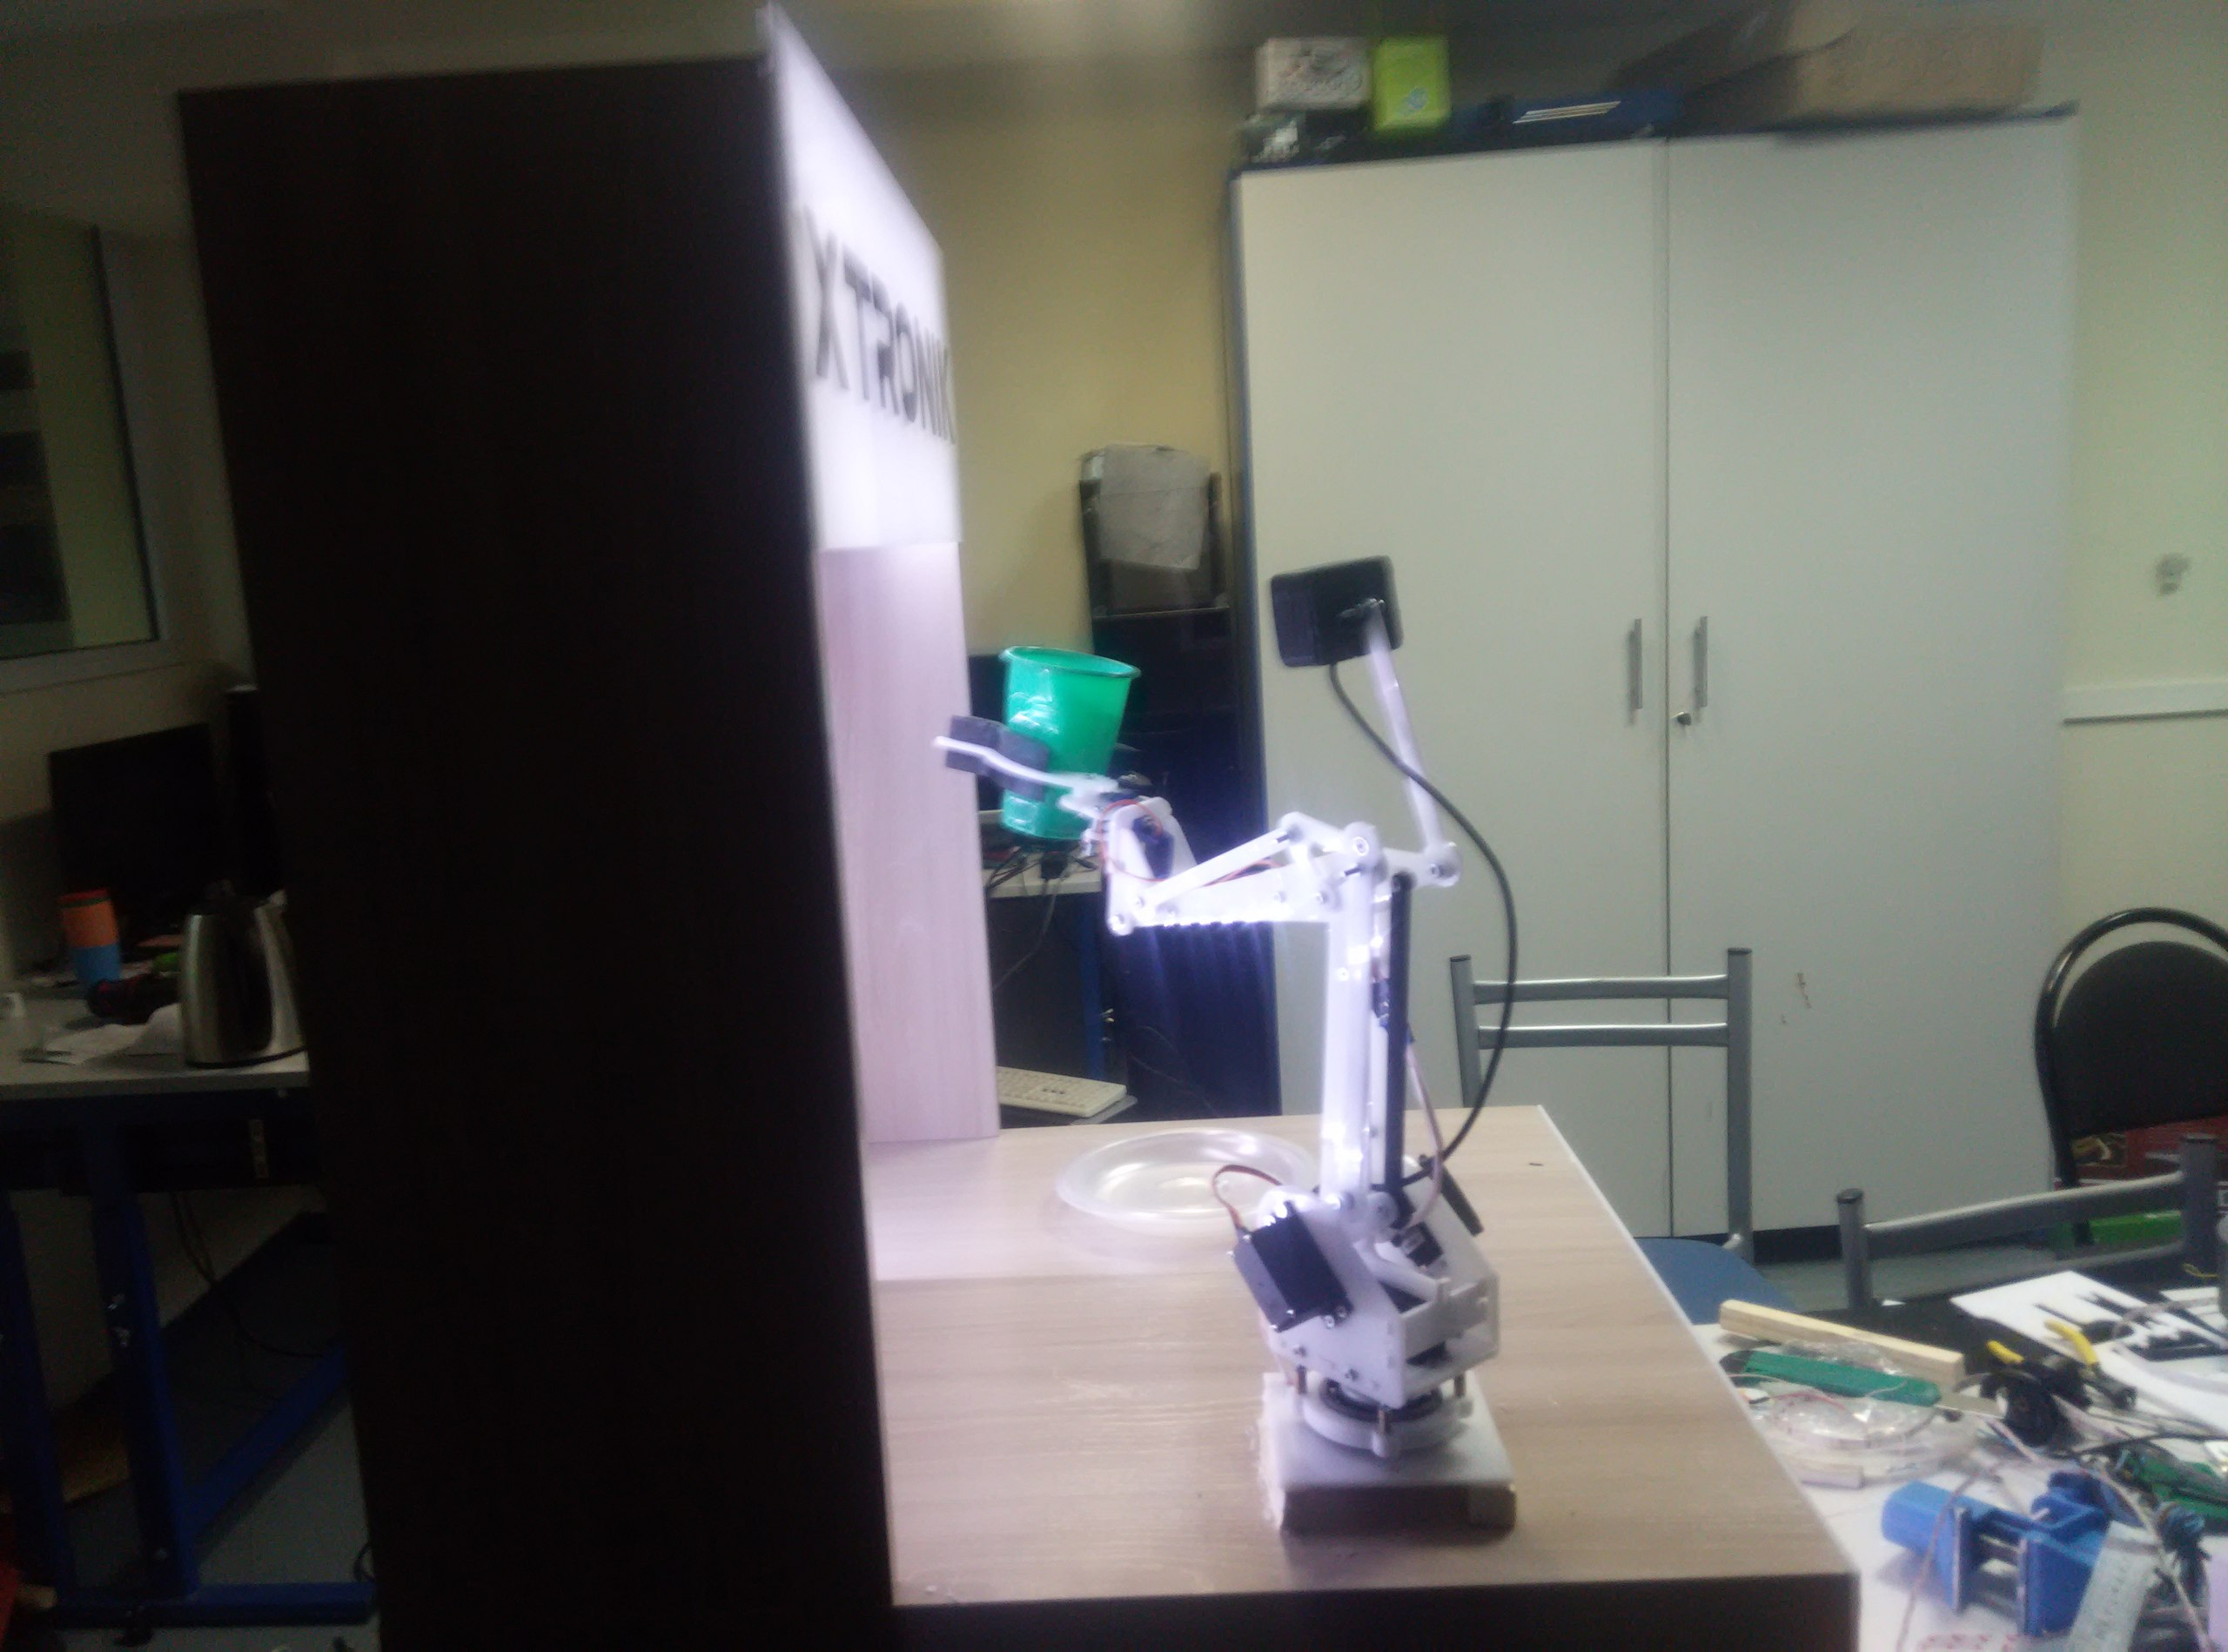
\includegraphics[width=0.85\linewidth]{images/sboku.jpg}}
\caption{Робот-повар. Вид сбоку}
\end{figure}

При испытании робота было обнаружены его недостатки:

\begin{itemize}
   	\item движения манипулятора не были плавными;
   	\item нахождение предмета сильно зависело от освещения;
   	\item захват предмета не всегда проходил успешно и в случае неудачи, манипулятор продолжал запрограммированные действия, будто предмет он захватил;
   	\item программа давала сбой и робот <<впадал в ступор>>.
\end{itemize}

Часть вышеперечисленного удалось исправить. Для улучшения процесса захвата, была поставлена более широкая <<клешня>>, а для более успешного нахождения были отредактированны параметры поиска. Сбои удалось исключить посредством улучшения качества программного кода.

Т.к. качество камеры было недостаточно высокое и сервоприводы были малой мощности, случаи незахвата предмета и ненахождения объекта остались, но были сведены к минимуму.

В финальной версии роботы выглядел, как на рисунке 6.2.

\begin{figure}[h!]
\center{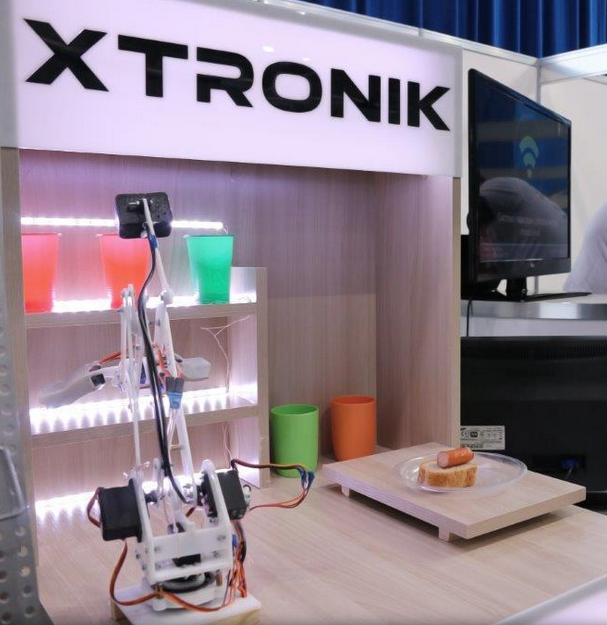
\includegraphics[width=0.85\linewidth]{images/vyst.png}}
\caption{Робот-повар в процессе сборки бутерброда}
\end{figure}

\newpage

<<Мир глазами робота>> представлен на рисунке 6.3.
 
\begin{figure}[h!]
\center{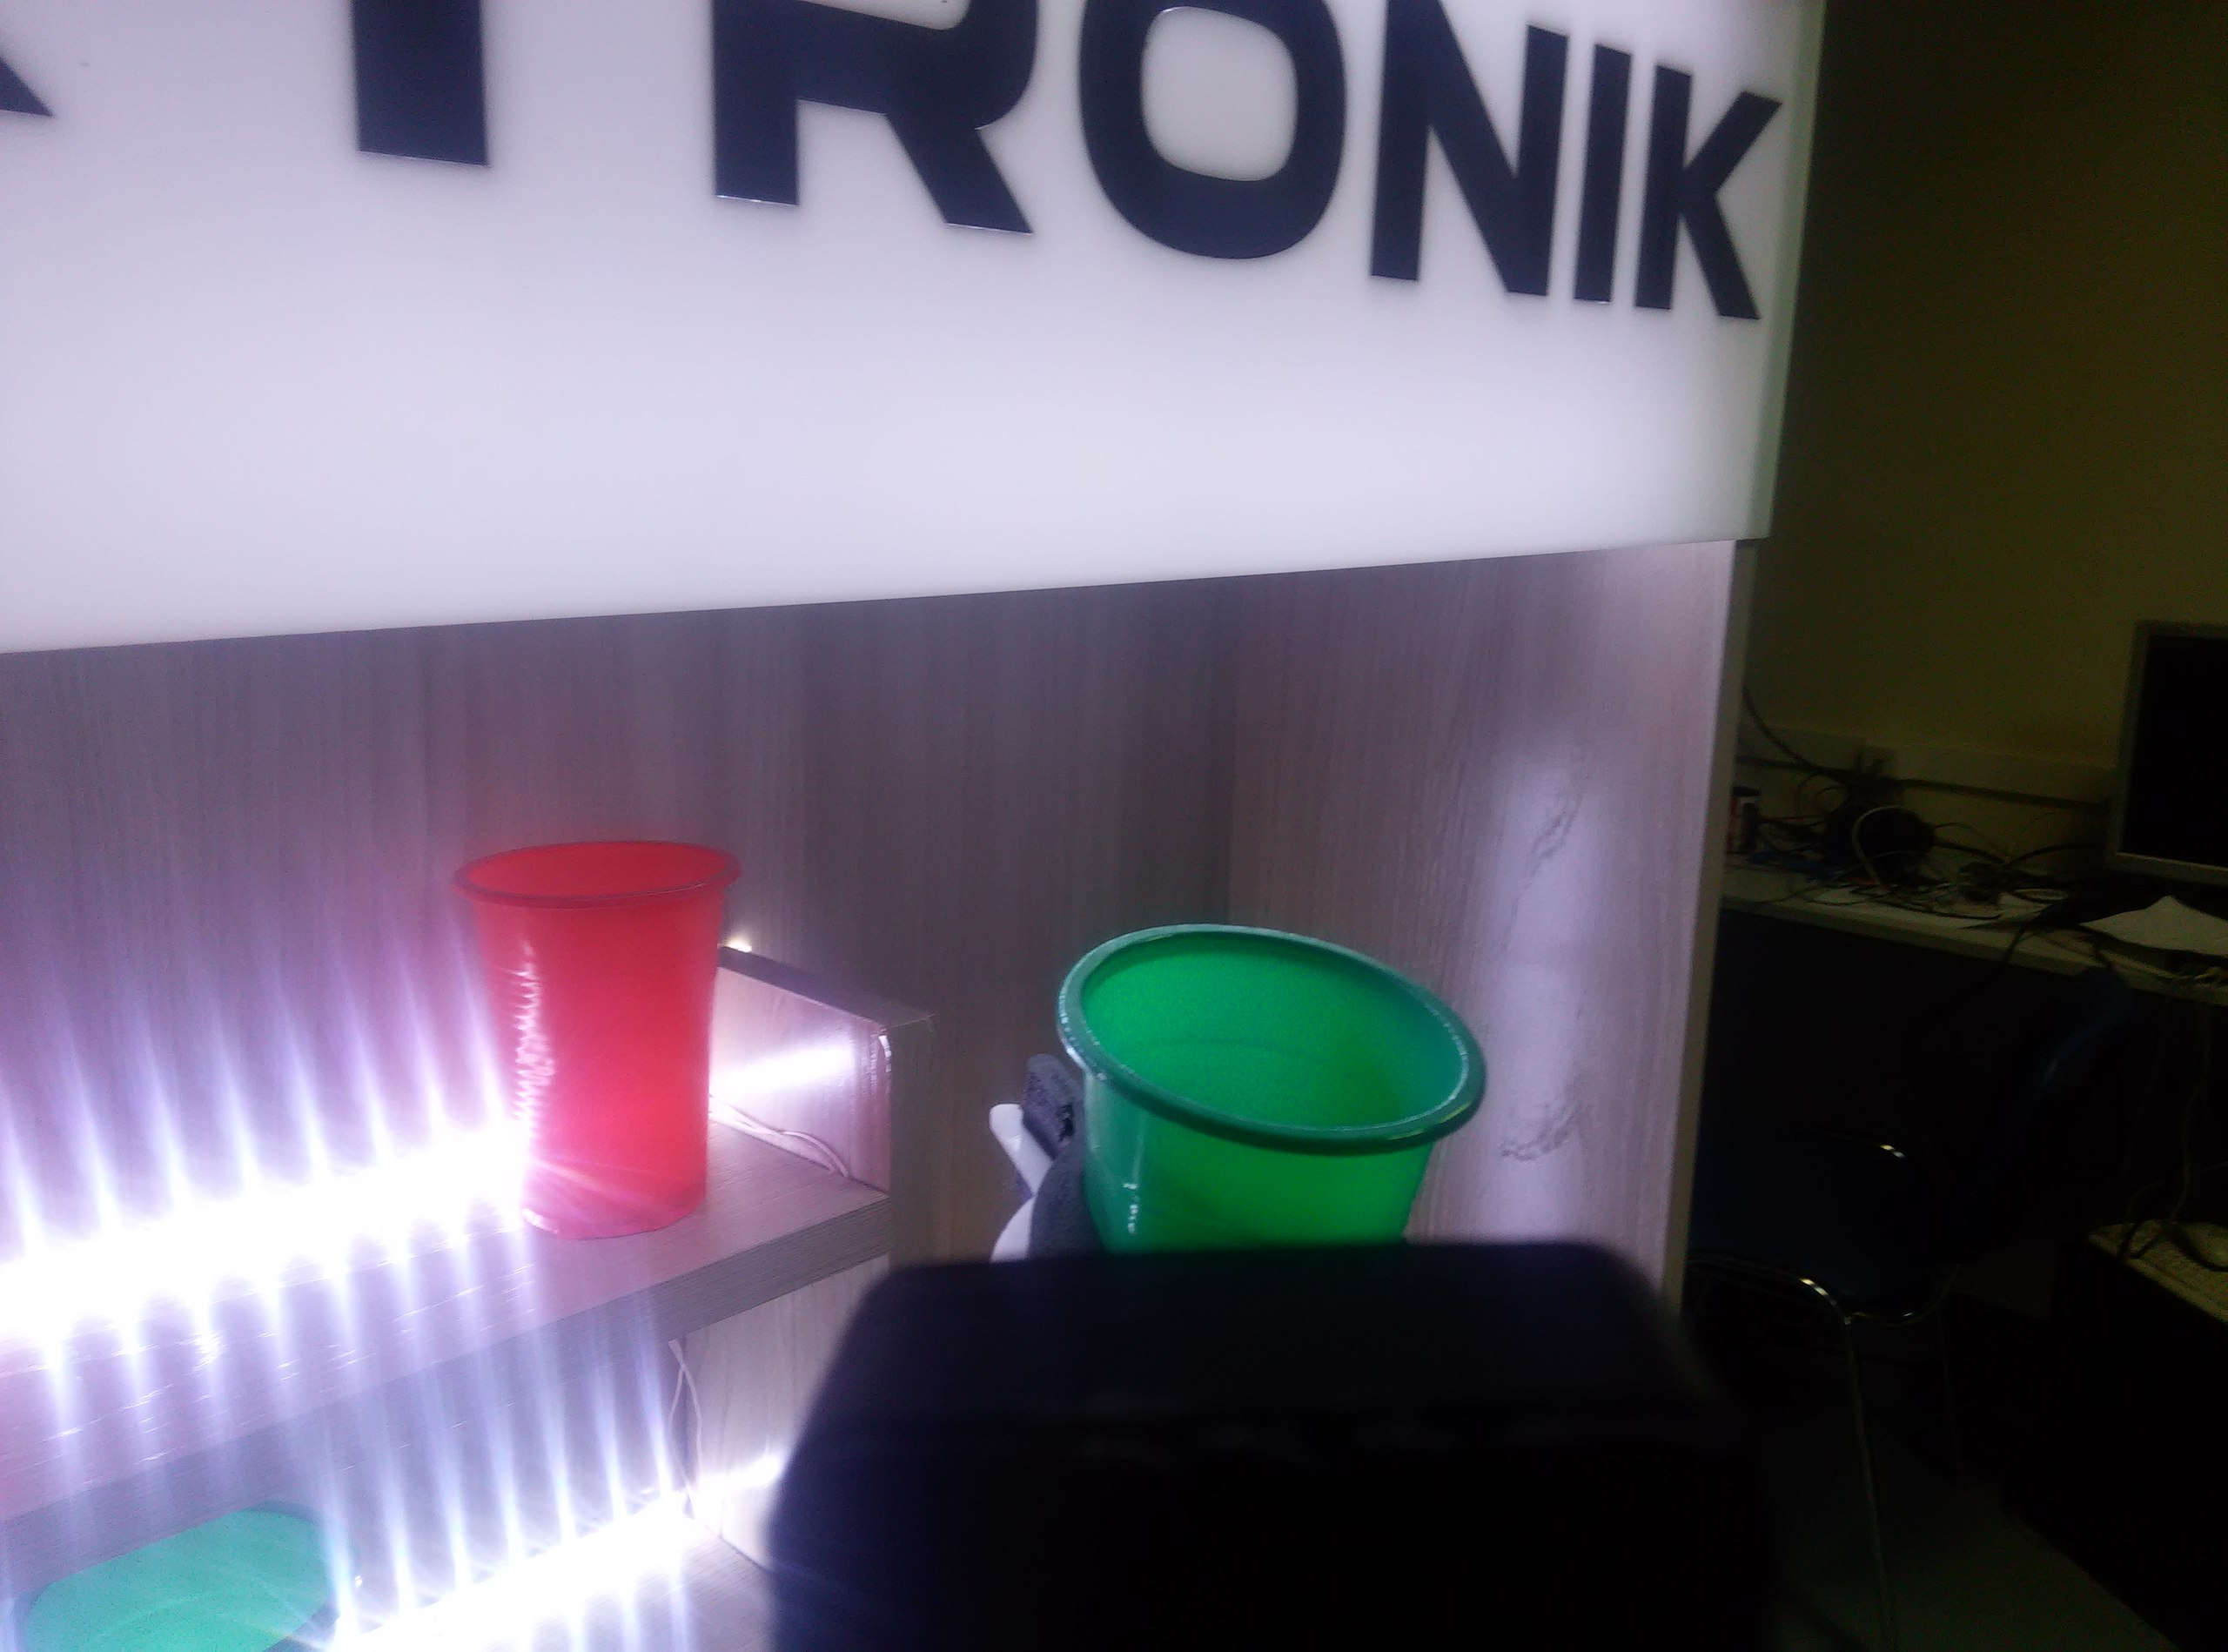
\includegraphics[width=0.85\linewidth]{images/webcam.jpg}}
\caption{Вид с вебкамеры}
\end{figure}
 \newpage
 \section{Заключение}
 В процессе прохождения производственной практики были получены навыки программирования с системой компьютерного зрения, навыки программирования микроконтроллеров arduino и передача информации по com-порту.

В ходе работы над проектом <<робота-повара>> были поняты некоторые недостатки и преимущества использованных библиотек и технологий.

Над данным проектом работало нескольно человек, поэтому были повышены навыки программирования в команде, чтение чужого программного кода. Также понята необходимость написание программ так, чтобы его могли прочитать другие сотрудники.
 \newpage
 \section*{Список используемых источников}
 \addcontentsline{toc}{section}{Список используемых источников}
 \begin{enumerate}
\item Промышленные манипуляторы. [Электронный ресурс]. Режим доступа:
https://ru.wikipedia.org/wiki/Промышленный\_робот (Дата обращения: 19.06.2016)

\item Машинное зрение. [Электронный ресурс]. Режим доступа:
https://ru.wikipedia.org/wiki/Машинное\_зрение (Дата обращения: 20.06.2016)

\item OpenCV. [Электронный ресурс]. Режим доступа:
https://ru.wikipedia.org/wiki/OpenCV (Дата обращения: 21.06.2016)

\item Основы программирования на Arduino. [Электронный ресурс]. Режим доступа:
http://developer.alexanderklimov.ru/arduino-minimum.php (Дата обращения: 18.06.2016)
\end{enumerate}
 \ESKDappendix{Справочное}{\normalfont Листинг программы}
\begin{lstlisting}

#include <opencv\cv.h>
#include <opencv\highgui.h>
#include <stdlib.h>
#include <stdio.h>
#include <iostream>
#include  <windows.h>
#include <iostream>
#include <string>
#include <math.h>
using namespace std;

#define BUFSIZE 255
unsigned char bufrd[BUFSIZE], bufwr[BUFSIZE];
HANDLE COMport;
OVERLAPPED overlapped;
unsigned long counter;


HANDLE hSerial;

IplImage* image = 0;
IplImage* frame=0;
IplImage* dst = 0;
IplImage* hsv = 0;
IplImage* h_plane = 0;
IplImage* s_plane = 0;
IplImage* v_plane = 0;
IplImage* h_range = 0;
IplImage* s_range = 0;
IplImage* v_range = 0;
IplImage* hsv_and = 0;
int CamFlagCol = 1;
int CamFlagCam = 1;

int Hmin = 0;
int Hmax = 256;
int Smin = 0;
int Smax = 256;
int Vmin = 0;
int Vmax = 256;
int HSVmax = 256;
int Servo = 50;
int Servo1 = 0;
int Servo2 = 0;
int Servo3 = 0;
int Servo4 = 90;
int Servo_S = 0;
int Servo2_S = 0;
int flag = 0;
int flag2 = 0;

bool Kl = false;
bool Cup = false;
bool Obj = false;
int xKl, yKl, xCup, yCup, xObj = 0, yObj = 0;

void peredacha(int x, int y, int a, int area, int l)
{
  char *str2 = new char[4];
  char *str = new char[1];
  int k = 0, s=0, shag=0;
  DWORD dwSize;
  DWORD dwBytesWritten;
  BOOL iRet;


  if (flag2 == 0){
    s=415-x;
    if(fabs(double (s))<15){shag=0; flag2=1; 
    	Servo_S=Servo;}else{shag=1;}
    if(fabs(double (s))>60) shag=5*shag; else if(fabs(double (
    	s))>40) shag=3*shag;
    if(s<0) shag=-1*shag;
    Servo=Servo+shag;
    if(Servo>180){Servo=180;}else if(Servo<0){Servo=0;}
  }else if(flag2 == 4){
    Servo=Servo-2;
    if(Servo<30){flag2 = 5;}
  }else if(flag2 == 7){
    Servo=Servo+2;
    if(Servo_S-Servo<3){flag2 = 8;}
  }
  itoa(Servo,str2,10);
  if(Servo<10){s=3;}else if(Servo<100){s=2;}else{s=1;}
  dwSize = sizeof(str2)-s;
  iRet = WriteFile (hSerial,str2,dwSize,&dwBytesWritten,NULL);
  iRet = WriteFile (hSerial,",",1,&dwBytesWritten,NULL);
  
  /*s=fabs(double (240-y));
  if(s<15){shag=0;}else{shag=1;}
  if(240-y<0) shag=-1*shag;
  Servo1=Servo1+shag;
  if(Servo1>180){Servo1=180;}else if(Servo1<0){Servo1=0;}
  itoa(Servo1,str2,10);
  if(Servo1<10){s=3;}else if(Servo1<100){s=2;}else{s=1;}
  itoa(y,str2,10);
  dwSize = sizeof(str2)-1;
  iRet = WriteFile (hSerial,"0",1,&dwBytesWritten,NULL);
  iRet = WriteFile (hSerial,",",1,&dwBytesWritten,NULL);

  if (flag2 == 2){
    Servo2=Servo2+10;
    if (Servo2==100) {flag2 = 3;}
  }else if(flag2==9){
    Servo2=Servo2-10;
    if (Servo2==0) {flag2 = 10;}
  }
  itoa(Servo2,str2,10);
  if(Servo2<10){s=3;}else if(Servo2<100){s=2;}else{s=1;}
  dwSize = sizeof(str2)-s;
  iRet = WriteFile (hSerial,str2,dwSize,&dwBytesWritten,NULL);
  iRet = WriteFile (hSerial,",",1,&dwBytesWritten,NULL);

  if (flag2 == 1){
    if((l<140)&&(l>0)){shag=0; flag2=2; 
    	Servo2_S=Servo3;}else{shag=1;}
    Servo3=Servo3+shag;
    if(Servo3>100){Servo3=100;}else if(Servo3<0){Servo3=0;}
  }else if (flag2 == 3){
    Servo3=Servo3-5;
    if(Servo3<5){flag2 = 4;}
  }else if(flag2 == 8){
    Servo3=Servo3+2;
    if(Servo2_S-Servo3<3){flag2 = 9;}
  }
  itoa(Servo3,str2,10);
  if(Servo3<10){s=3;}else if(Servo3<100){s=2;}else{s=1;}
  dwSize = sizeof(str2)-s;
  iRet = WriteFile (hSerial,str2,dwSize,&dwBytesWritten,NULL);
  iRet = WriteFile (hSerial,",",1,&dwBytesWritten,NULL);

  if (flag2 == 5){
    Servo4=Servo4+10;
    if(Servo4==180){flag2 = 6;}
  }else if (flag2 == 6){
    Servo4=Servo4-10;
    if(Servo4==90){flag2 = 7;}
  }
  itoa(Servo4,str2,10);

  if(Servo4<10){s=3;}else if(Servo4<100){s=2;}else{s=1;}
  dwSize = sizeof(str2)-s;
  iRet = WriteFile (hSerial,str2,dwSize,&dwBytesWritten,NULL);
  iRet = WriteFile (hSerial,";",1,&dwBytesWritten,NULL);

  cout << Servo << ","<< Servo1 << ","<< Servo2 << ","
  << Servo3 << ";" <<endl;
}

void funcColour(int fkey=0){
  if (fkey == 119) CamFlagCol = 1;
  else if (fkey == 114) CamFlagCol = 2;
  else if (fkey == 103) CamFlagCol = 3;
  else if (fkey == 120) CamFlagCol = 4;

  if (CamFlagCam == 1){
  // White
  if (CamFlagCol == 1){
    Hmin = 0;
    Hmax = 191;
    Smin = 0;
    Smax = 45;
    Vmin = 188;
    Vmax = 255;
    flag = 0;
  }
  // Red
  if (CamFlagCol == 2){
    Hmin = 0;
    Hmax = 20;
    Smin = 115;
    Smax = 256;
    Vmin = 100;
    Vmax = 197;  
    flag = 0;
  }
  // Green
  if (CamFlagCol == 3){
    Hmin = 39;
    Hmax = 76;
    Smin = 73;
    Smax = 256;
    Vmin = 33;
    Vmax = 187;
    flag = 0;
  }
    // Temp colour
  if (CamFlagCol == 4){
    Hmin = 78;
    Hmax = 130;
    Smin = 87;
    Smax = 256;
    Vmin = 100;
    Vmax = 256;
    flag = 0;
  }
  }
  if (CamFlagCam == 2){
  // White
  if (CamFlagCol == 1){
    Hmin = 0;
    Hmax = 191;
    Smin = 0;
    Smax = 45;
    Vmin = 188;
    Vmax = 255;
    flag = 0;
  }
  // Red
  if (CamFlagCol == 2){
    Hmin = 159;
    Hmax = 181;
    Smin = 181;
    Smax = 255;
    Vmin = 52;
    Vmax = 256;  
    flag = 0;
  }
  // Green
  if (CamFlagCol == 3){
    Hmin = 39;
    Hmax = 76;
    Smin = 73;
    Smax = 256;
    Vmin = 33;
    Vmax = 187;
    flag = 0;
  }
    // Temp colour
  if (CamFlagCol == 4){
    Hmin = 78;
    Hmax = 130;
    Smin = 87;
    Smax = 256;
    Vmin = 100;
    Vmax = 256;
    flag = 1;
  }
  }
  if (CamFlagCam == 3){
  // 
  Hmin = 64;
  Hmax = 117;
  Smin = 29;
  Smax = 101;
  Vmin = 200;
  Vmax = 256;  
  flag = 0;
  }

}

void funcCvIn(){
  cvInRangeS(h_plane, cvScalar(Hmin), cvScalar(Hmax), h_range);
  cvInRangeS(h_plane, cvScalar(Hmin), cvScalar(Hmax), h_range);
  cvInRangeS(s_plane, cvScalar(Smin), cvScalar(Smax), s_range);
  cvInRangeS(s_plane, cvScalar(Smin), cvScalar(Smax), s_range);
  cvInRangeS(v_plane, cvScalar(Vmin), cvScalar(Vmax), v_range);
  cvInRangeS(v_plane, cvScalar(Vmin), cvScalar(Vmax), v_range);
}

int ac = 0;

int WhTr(CvCapture* capture, double width, double height, int 
	counter, int No){
  char filename[512];
  int AB, AC;
  float area, perim, l;
  if (Obj == false) {xObj = 0;}


  if (No == 1)
  CamFlagCam = 1;
  else
  {
    CamFlagCam = 2+ac;
    if (ac == 0) ac = 1;
    else ac = 0;
  }

  funcColour();

  frame = cvQueryFrame( capture );
    
  image = frame;
  hsv = cvCreateImage( cvGetSize(image), IPL_DEPTH_8U, 3 );
  h_plane = cvCreateImage( cvGetSize(image), IPL_DEPTH_8U, 1 );
  s_plane = cvCreateImage( cvGetSize(image), IPL_DEPTH_8U, 1 );
  v_plane = cvCreateImage( cvGetSize(image), IPL_DEPTH_8U, 1 );
  h_range = cvCreateImage( cvGetSize(image), IPL_DEPTH_8U, 1 );
  s_range = cvCreateImage( cvGetSize(image), IPL_DEPTH_8U, 1 );
  v_range = cvCreateImage( cvGetSize(image), IPL_DEPTH_8U, 1 );
  hsv_and = cvCreateImage( cvGetSize(image), IPL_DEPTH_8U, 1 );
  cvCvtColor( image, hsv, CV_BGR2HSV ); 
  cvCvtPixToPlane( hsv, h_plane, s_plane, v_plane, 0 );
  
  if (No == 1)
    cvNamedWindow("hsv and 1",CV_WINDOW_AUTOSIZE);
  else
    cvNamedWindow("hsv and 2",CV_WINDOW_AUTOSIZE);

  funcCvIn();
  cvAnd(h_range, s_range, hsv_and);
  cvAnd(hsv_and, v_range, hsv_and);

  dst = cvCloneImage(hsv_and);
  cvErode(dst, dst, 0, 5);

  CvMemStorage* storage = cvCreateMemStorage(0);
  CvSeq* contours=0;

  int contoursCont = cvFindContours(dst, storage,&contours,
  	sizeof(CvContour),CV_RETR_EXTERNAL,CV_CHAIN_APPROX_TC89_KCOS,
  	cvPoint(0,0));
  if (contours!=0)contours = cvApproxPoly( contours, sizeof(
  	CvContour), storage, CV_POLY_APPROX_DP, 1, 1);

  if (CamFlagCam == 2) Cup = false;
  else if (CamFlagCam == 3) Kl = false;
    

  for( CvSeq* current = contours; current != NULL; current = 
  	current->h_next ){
    area = fabs(cvContourArea(current));
    perim = cvContourPerimeter(current);
    if ( (area > 200.0) && (fabs(perim - 2*(width+height)) > 50.0  
    	) ){
      cvDrawContours(frame, current, cvScalar(0, 0, 255), 
      	cvScalar(0, 255, 0), 0, 3, 8);
      CvRect rect;
      CvPoint pt1, pt2;
      rect=cvBoundingRect(current, NULL);
      pt1.x = rect.x;
      pt2.x = (rect.x+rect.width);
      pt1.y = rect.y;
      pt2.y = (rect.y+rect.height);
        
      int xA = pt1.x;
      int xD = pt2.x;
      int yA = pt1.y;
      int yD = pt2.y;
      int xB = xD;
      int yB = yA;
      int xC = xA;
      int yC = yD;
      int AB = int ((xA + xB)/2);
      int AC = int ((yA + yC)/2);

      if (No == 1){
        xObj = AB;
        yObj = AC;
        Obj = true;
      }

      if (No == 2)
        if (CamFlagCam == 2){
        Cup = true;
        xCup = AB;
        yCup = AC;
        }
        if (CamFlagCam == 3) {
        Kl = true;
        xKl = AB;
        yKl = AC;
        }

    }
  }
  if  (No==1)  cvShowImage("capture1", frame);
  if  (No==2)  cvShowImage("capture2", frame);


  cvReleaseMemStorage(&storage);


  cvErode(hsv_and, hsv_and, NULL, 3);
  cvDilate(hsv_and, hsv_and, NULL, 1);

  char c = cvWaitKey(33);
  if (c == 27) { 
    return(1);
  }
  else if(c == 13) { 
    sprintf(filename, "Image%d.jpg", counter);
    printf("[i] capture... %s\n", filename);
    cvSaveImage(filename, frame);
    counter++;
  }
  funcColour(c);

  
  if (No==1) cvShowImage( "hsv and 1", hsv_and );
  if (No==2) cvShowImage( "hsv and 2", hsv_and );

  if (Cup && Kl){  
    l = sqrt(pow((xKl-xCup),2) + pow((yKl-yCup),2));
    if (l < 170){
    }
  }
  else printf("\n");
  if (flag == 1){ 
    peredacha(xObj, yObj, area, area, l);
  
  }
  cvReleaseImage( &h_plane );
  cvReleaseImage( &s_plane );
  cvReleaseImage( &v_plane );
  cvReleaseImage( &h_range );
  cvReleaseImage( &s_range );
  cvReleaseImage( &v_range );
  cvReleaseImage( &hsv );
  cvReleaseImage( &hsv_and );
  cvReleaseImage( &dst);

  return(0);
}

int func1(){
  CvCapture* capture = cvCaptureFromCAM( 1 );
  CvCapture* Scapture = cvCaptureFromCAM( 2 );
    

    double width = cvGetCaptureProperty(capture, 
    	CV_CAP_PROP_FRAME_WIDTH);
    double height = cvGetCaptureProperty(capture, 
    	CV_CAP_PROP_FRAME_HEIGHT);
  printf("[i] #1 %.0f x %.0f\n", width, height );
    double Swidth = cvGetCaptureProperty(Scapture, 
    	CV_CAP_PROP_FRAME_WIDTH);
    double Sheight = cvGetCaptureProperty(Scapture, 
    	CV_CAP_PROP_FRAME_HEIGHT);
  printf("[i] #2 %.0f x %.0f\n", Swidth, Sheight );

    
  
    cvNamedWindow("capture1", CV_WINDOW_AUTOSIZE);
    cvNamedWindow("capture2", CV_WINDOW_AUTOSIZE);

    printf("[i] press Enter for capture image and Esc for 
    	quit!\n");

    int counter=0;

  while(true) {
    if (WhTr(capture, width, height, counter, 1)==1) break;
    if (WhTr(Scapture, Swidth, Sheight, counter, 2)==1) break;
  }
    cvReleaseCapture( &capture );  
    cvDestroyAllWindows();
  printf("-----\n");

  return(0);
}

int main(int argc, char* argv[])
{
  LPCTSTR sPortName = L"COM5";
  hSerial = ::CreateFile(sPortName,GENERIC_READ | 
  GENERIC_WRITE,0,0,OPEN_EXISTING,FILE_ATTRIBUTE_NORMAL,0);
  if(hSerial==INVALID_HANDLE_VALUE)
  {
    if(GetLastError()==ERROR_FILE_NOT_FOUND)
  {
    cout << "serial port does not exist.\n";
  }
  cout << "some other error occurred.\n";
  }
  
  DCB dcbSerialParams = {0};
  dcbSerialParams.DCBlength=sizeof(dcbSerialParams);
  if (!GetCommState(hSerial, &dcbSerialParams))
  {
  cout << "getting state error\n";
  }
  
  dcbSerialParams.BaudRate=CBR_9600;
  dcbSerialParams.ByteSize=8;
  dcbSerialParams.StopBits=ONESTOPBIT;
  dcbSerialParams.Parity=NOPARITY;
  if(!SetCommState(hSerial, &dcbSerialParams))
  {
  cout << "error setting serial port state\n";
  }

  printf("Hello world!\nWrite 0 for exit\n    1 for main 
  	program\n    2 for choise param. HSV\n-----\n");
  int key;
  while(true){
    printf("--> ");
    scanf("%d",&key);
    printf("\n");
    if (key == 0) return 0;
    else if (key == 1) func1();
    else if (key == 2) func2();
  }
    return 0;
}

\end{lstlisting}
 \newpage
 \end{document}